\chapter{Climate Risks}

Before going straight 
on climate risks, we need to agree on 
the definition of \textit{risk} in Finance. Suppose 
that a stock return follows an AR(1) process:

\begin{equation}
    R_{t} = \phi R_ {t-1} + \varepsilon_{t}
\end{equation}

with $\varepsilon_{t}$ is a \textit{white noise} process,
like a coin flip: completely unpredictable.
We generaly consider 
that it is 
mean zero $E_t(\varepsilon_{t+1}) = E(\varepsilon_{t+1}) = 0$
and constant variance $\sigma_t(\varepsilon_{t+1}) = \sigma(\varepsilon_{t+1})= \sigma_{\varepsilon}^2$.
Such white noise is also unpredictable from its past:
the \textit{autocorrelation} $\text{Corr}(\varepsilon_{t},\varepsilon_{t+1})=0$.
Below is an example of such white noise process.

\begin{figure}[htbp]
    \centering
    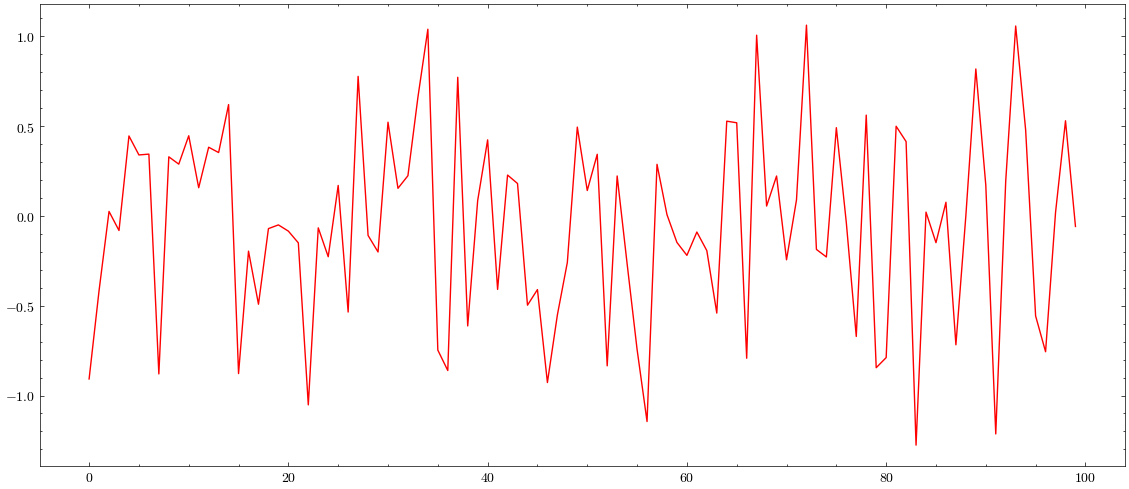
\includegraphics[width=1\textwidth]{../images/chapter01/unexpected_shocks.png}
    \caption{$\varepsilon_t$ with $\sigma_{\varepsilon} = 0.5$}
    \label{fig:fig01}
\end{figure}


The conditional expectation of the stock return is:

\begin{equation}
    \begin{aligned}
    E_t(R_{t+1}) = \phi R_t + E_t(\varepsilon_{t+1}) \\
    = \phi R_t
    \end{aligned}
\end{equation}

because $E_t(\varepsilon_{t+1}) = 0$.

The actual or \textit{realized} return will vary 
around this expectation. The unexpected return is:

\begin{equation}
    \begin{aligned}
    R_{t+1} - E_t(R_{t+1}) = \phi R_t + \varepsilon_{t+1} - \phi R_t \\
    = \varepsilon_{t+1}
    \end{aligned}
\end{equation}

and conditional variance of the stock return is:

\begin{equation}
    \begin{aligned}
    \sigma_t^2(R_{t+1}) = \sigma^2_t(\varepsilon_{t+1}) \\
    = \sigma_{\varepsilon}^2
    \end{aligned}
\end{equation}

due to the definition of the white noise 
process with constant variance, and the fact that
we already know $R_t$ at time $t$, so 
$\sigma_t^2(R_{t}) = 0$.

Risk is the unexpected in Finance. This 
is the fact that returns are not 
what we expected. Either higher or lower.
So, what matters is this $\varepsilon_{t+1}$ in 
our stock return process and its variance $\sigma_{\varepsilon}^2$.

\begin{figure}[htbp]
    \centering
    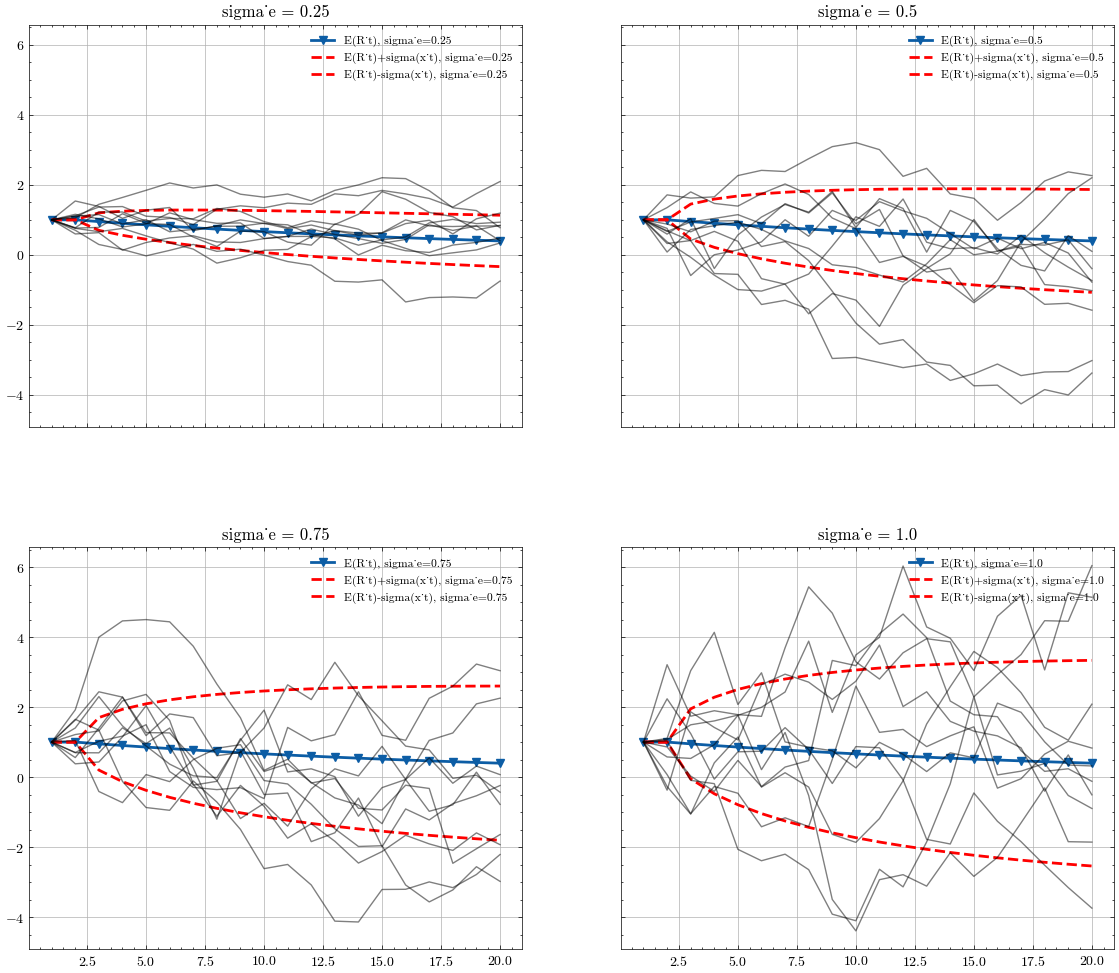
\includegraphics[width=1\textwidth]{../images/chapter01/ar_1.png}
    \caption{Simulation with increasing 
    uncertainty ($\sigma_{\varepsilon}^2$) in an AR(1) process.}
    \label{fig:fig01}
\end{figure}

Figure~\ref{fig:fig01} shows the stock return process
with increasing uncertainty $\sigma_{\varepsilon}^2$.
The more uncertain the process, the more
the realized returns will vary around the
expected returns. 

With this in mind, we can now move to the question 
of climate risks. 

\section{Climate Risks and Unexpected Returns}

With a simple one-period model, we can
show how climate change-related issues can add uncertainty
to asset prices (thus, risks).
We will consider two channels through which
climate change adds uncertainty: the cash-flows channel
and the discount rate channel.

\subsection{Cash-Flows Channel}

Let's define a payoff $X_{t+1}$ as the 
cash-flows provided to the investors per dollar invested in the stock at time $t$:

\begin{equation}
    X_{t+1} = \frac{CF_{t+1}}{P_t}
\end{equation}

Analysts form forecasts 
about the future cash-flows of the firm
based on information available at time $t$.
The expectations of the payoff
are a function of climate-related
conditions $CC_{t+1}$. $CC_{t+1}$ could represents 
any climate-related issues that may affect the
firm's cash-flows. But to make the things more 
concrete, we can think of $CC_{t+1}$ as 
a carbon tax. 
The expected payoff is then:

\begin{equation}
    E_t(X_{t+1}) = \beta_{cc} E_t(CC_{t+1})
\end{equation}

with $\beta_{cc}$ the sensitivities of 
the payoff to the carbon tax. Of course,
the payoff may also depend on other factors
like macroeconomic conditions. But 
for the sake of simplicity, we will focus
on the carbon tax example.
In order to forecast the future payoff, analysts 
needs to forecast future carbon tax
$E_t(CC_{t+1})$.

Suppose that the carbon tax $CC_{t+1}$ is an AR(1) process:

\begin{equation}
    CC_{t+1} = \phi CC_t + \tilde{CC}_{t+1}
\end{equation}

with $\tilde{CC}_{t+1}$ a white noise process
representing unexpected changes in the carbon tax.
Again, $E_t(\tilde{CC}_{t+1}) = 0$ and
$\sigma_t^2(\tilde{CC}_{t+1}) = \sigma_{\tilde{CC}}^2$.
The expected value of the carbon tax at time $t+1$ is:

\begin{equation}
    E_t(CC_{t+1}) = \phi CC_t
\end{equation}


\begin{figure}[htbp]
    \centering
    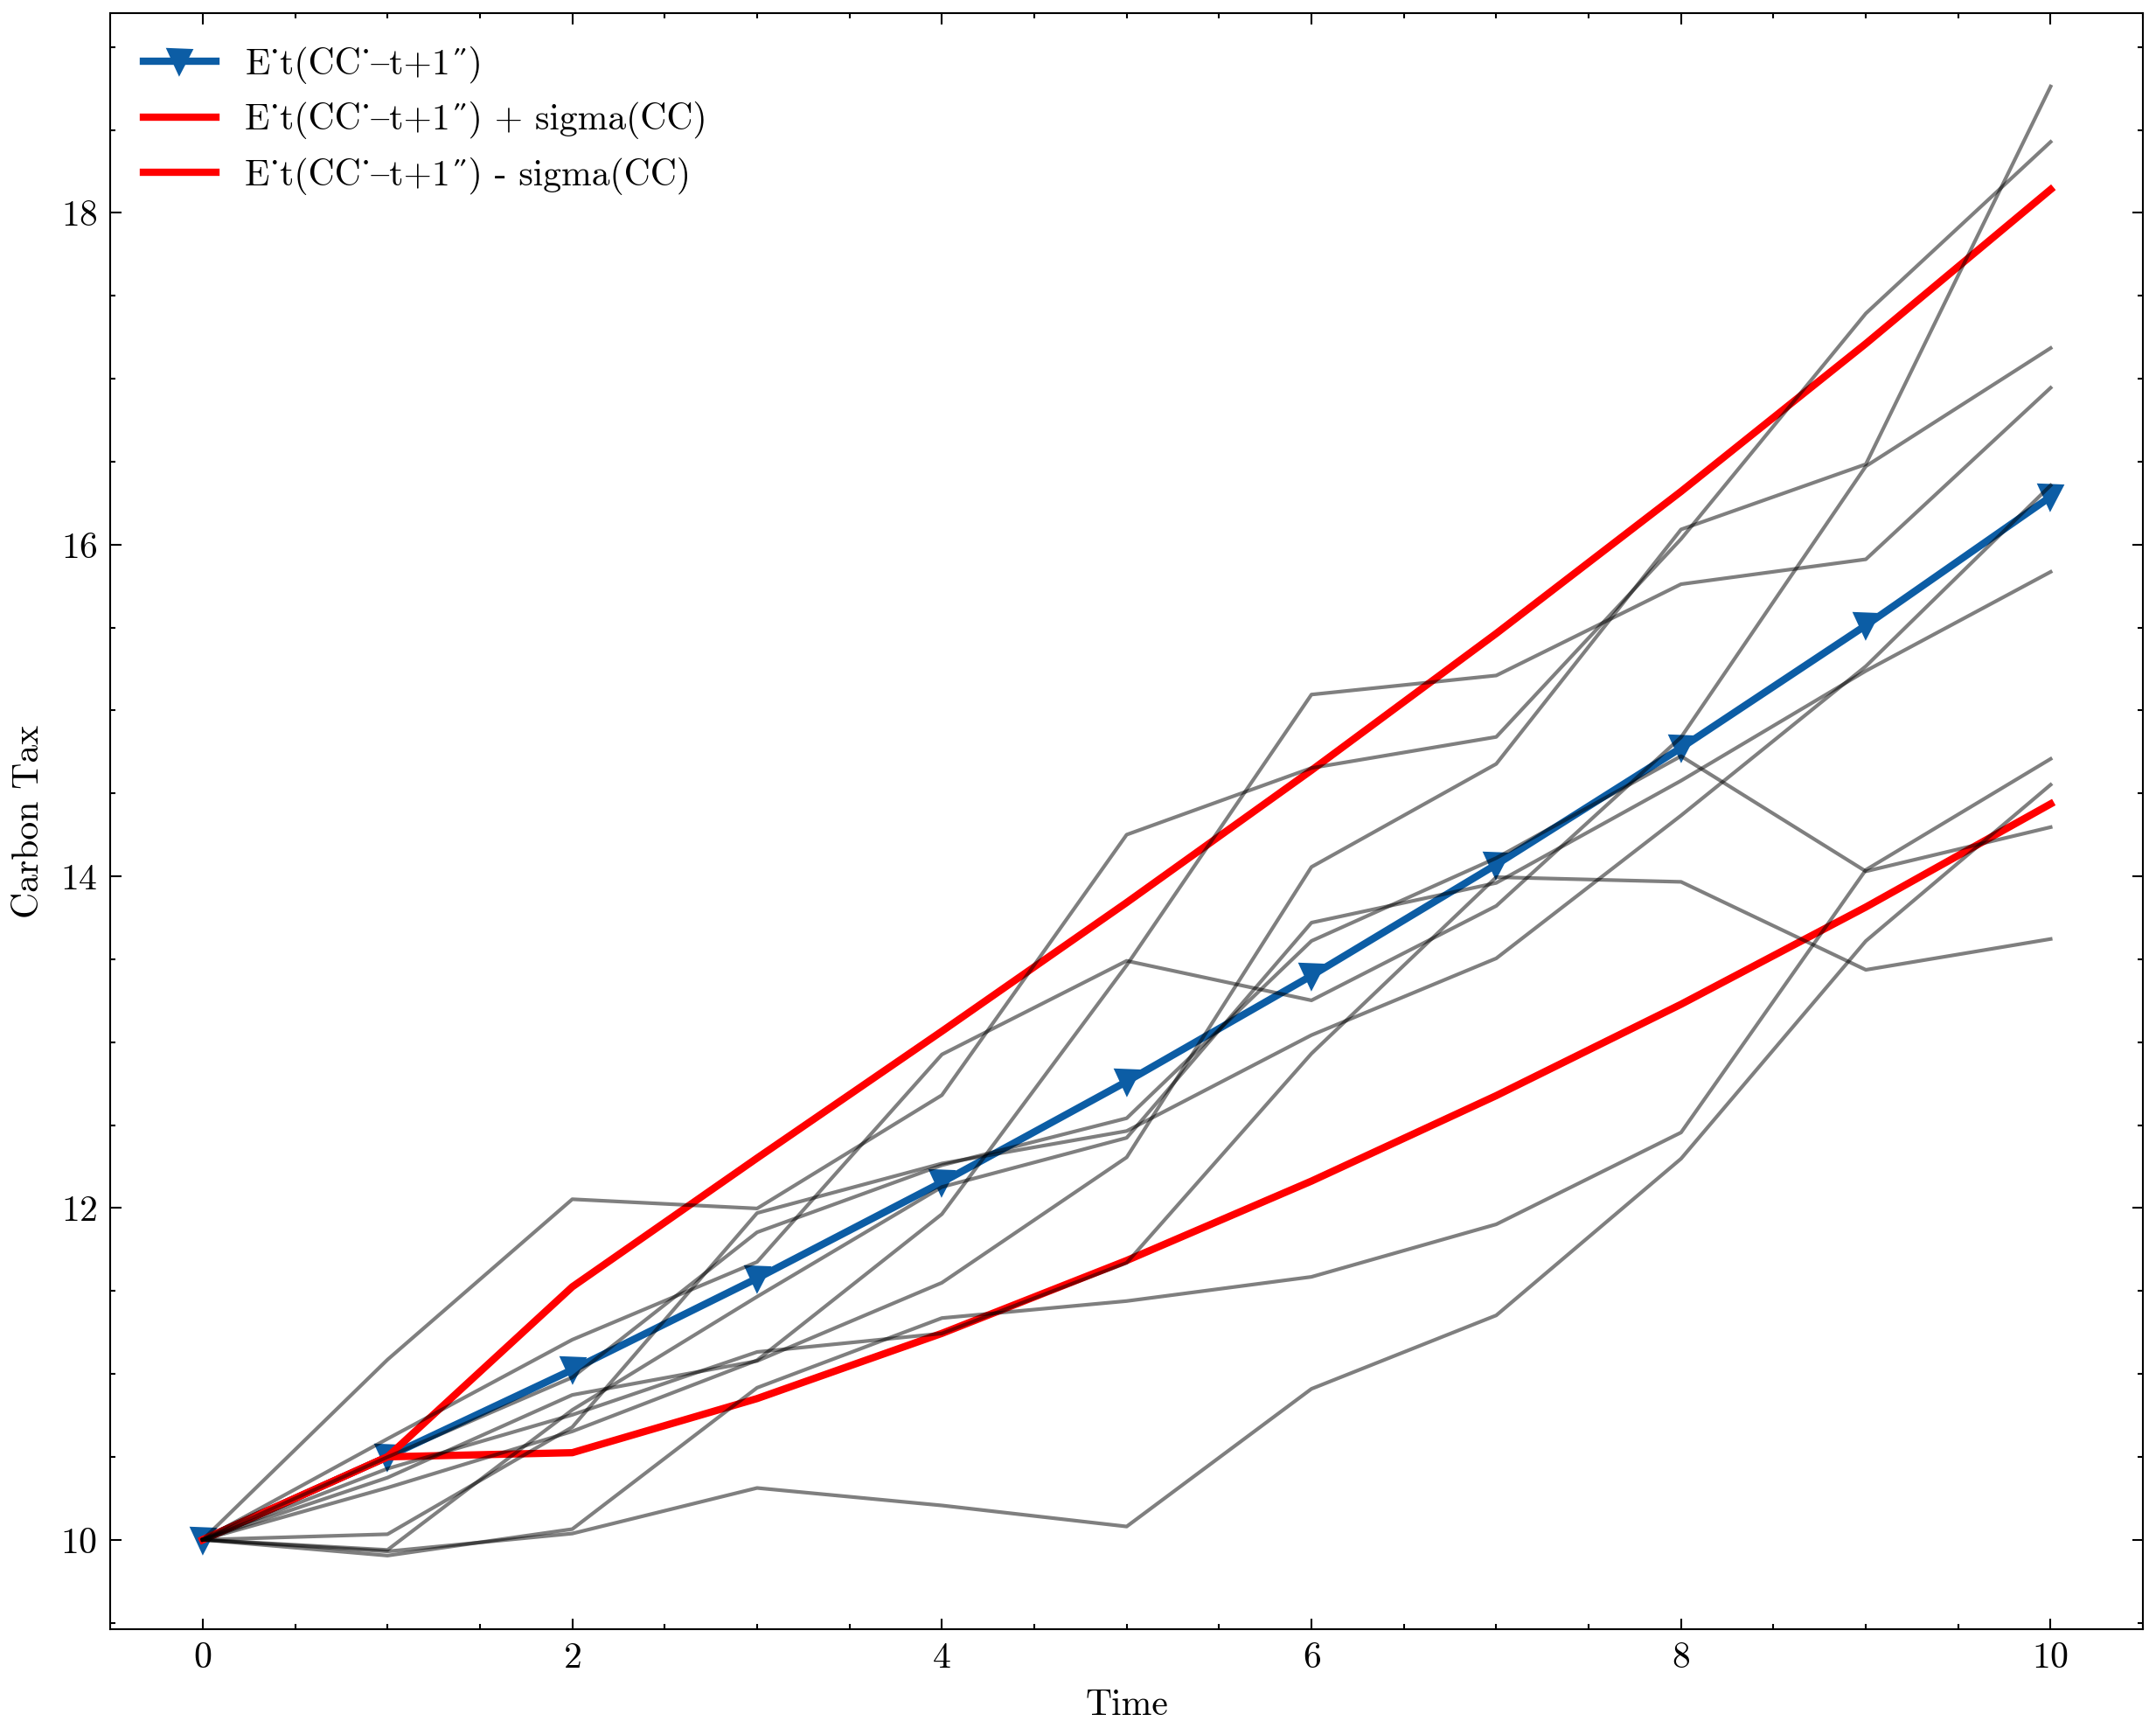
\includegraphics[width=0.8\textwidth]{../images/chapter01/carbon_tax_simulations.png}
    \caption{Simulation of the carbon tax process.}
    \label{fig:carbon_tax}
\end{figure}

The analysts may for example think that the carbon 
tax is supposed to increase by 5\%.
For the sake of the illustration, 
we simulate the carbon tax process with
$\phi = 1.05$ and $\sigma_{\tilde{CC}}^2 = 0.25$
with 10 periods
in figure~\ref{fig:carbon_tax} shows the carbon tax process.



Due to the possibility of unanticipated changes 
to the carbon tax,
the realized payoff may also differ from the expected one:

\begin{equation}
    X_{t+1} - E_{t}(X_{t+1}) = \beta_{CC} \tilde{CC}_{t+1} + \varepsilon_{t+1}
\end{equation}

Therefore, we can say that 
carbon tax uncertainty adds uncertainty to the
payoff, because:


\begin{figure}[htbp]
    \centering
    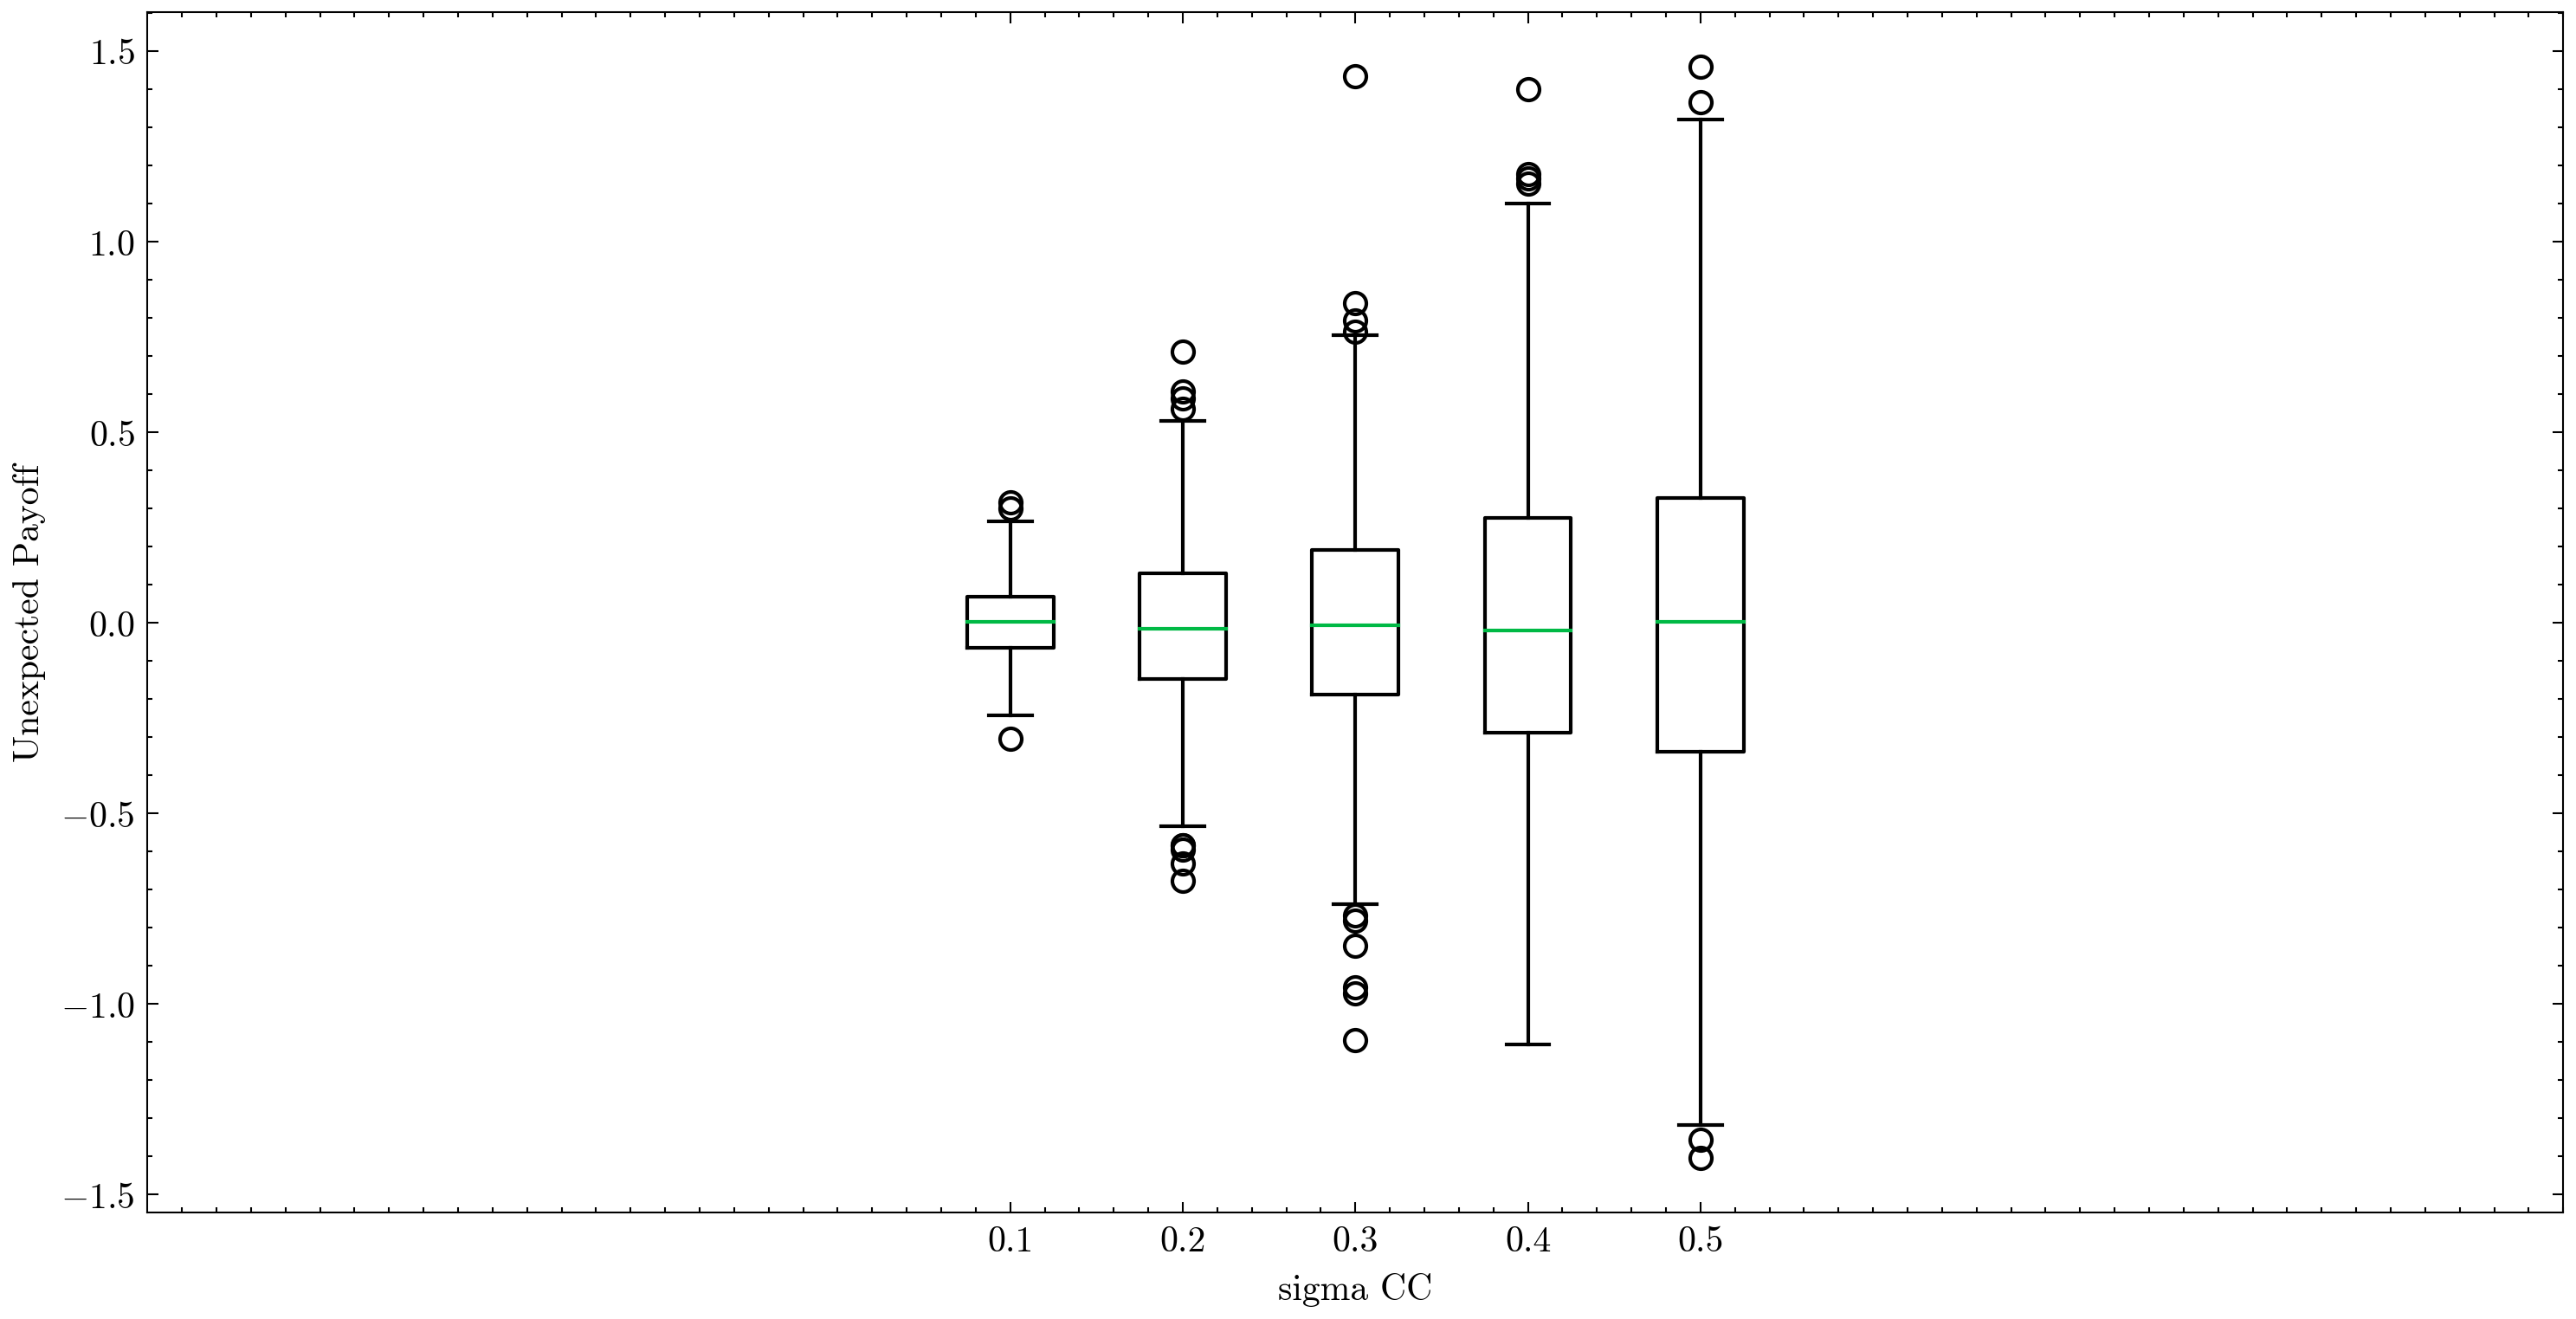
\includegraphics[width=0.8\textwidth]{../images/chapter01/unexpected_payoff_boxplot.png}
    \caption{Simulation of the unexpected payoff with different values for $\sigma_{\tilde{CC}}^2$.}
    \label{fig:payoff}
\end{figure}

\begin{figure}[htbp]
    \centering
    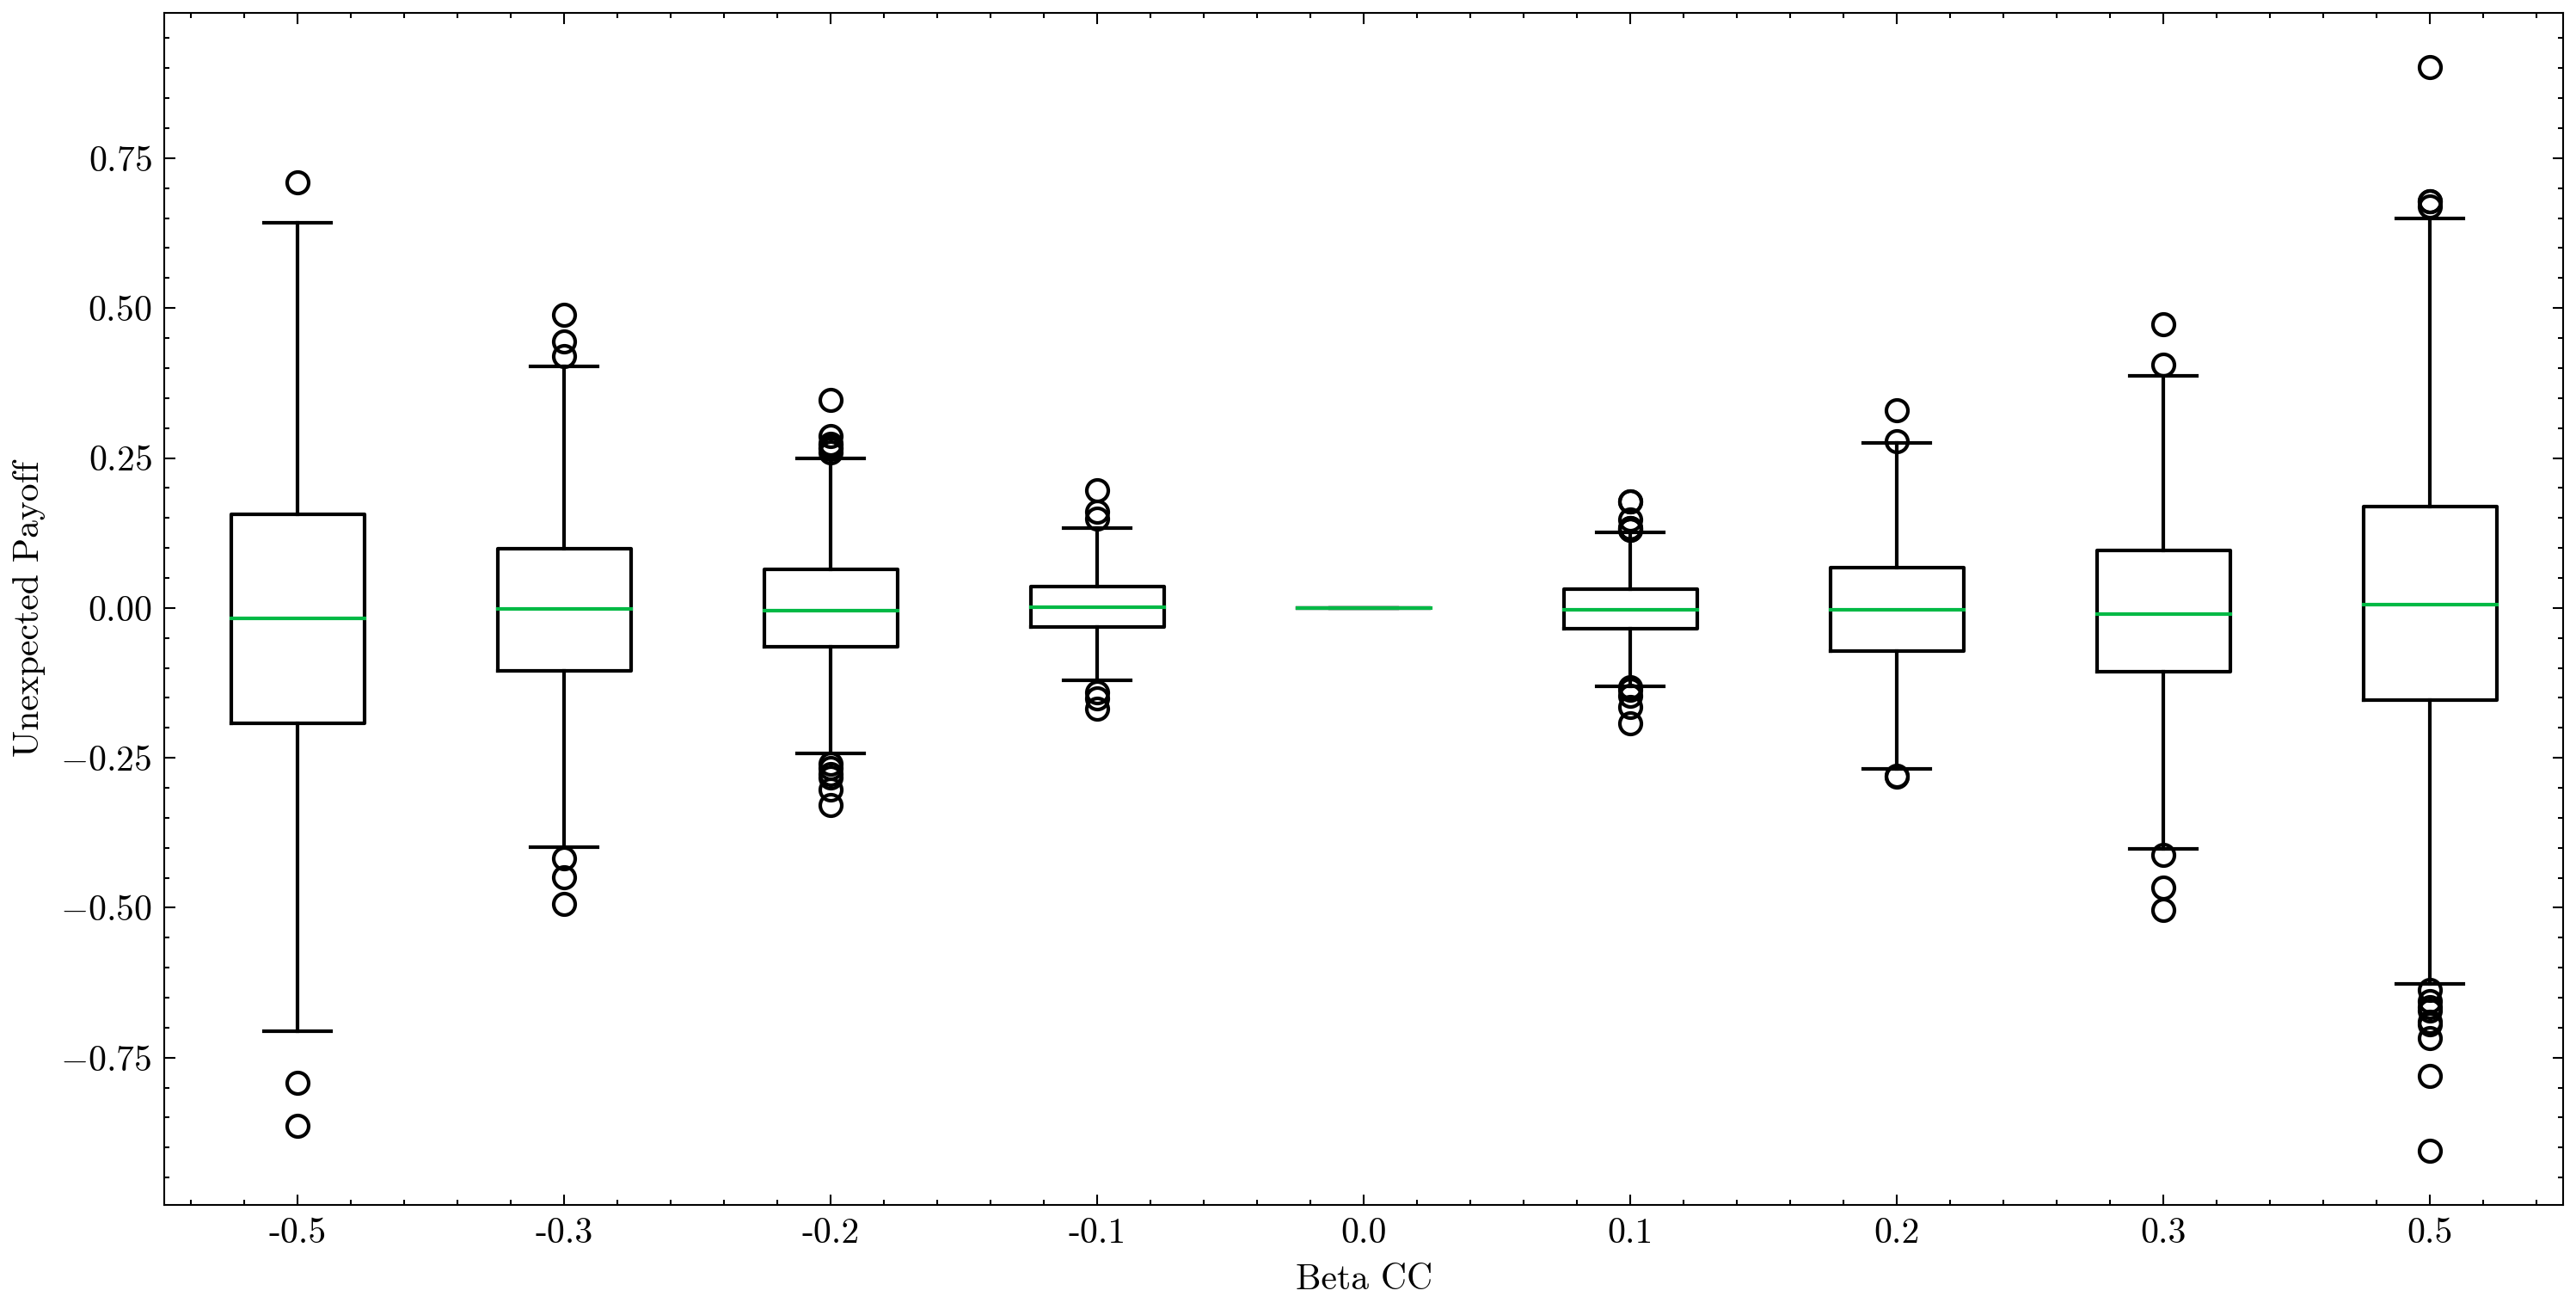
\includegraphics[width=0.8\textwidth]{../images/chapter01/unexpected_payoff_beta_cc.png}
    \caption{Simulation of the unexpected payoff with different values for $\beta_{CC}$.}
    \label{fig:payoff_beta}
\end{figure}



\begin{itemize}
    \item The highest the uncertainty in the carbon tax process ($\sigma_{\tilde{CC}}^2$),
    the more the realized payoff will vary around the expected payoff (see figure~\ref{fig:payoff}).
    \item The higher the sensitivity of the payoff to the carbon tax ($\beta_{CC}$),
    the more the realized payoff will vary around the expected payoff (see figure~\ref{fig:payoff_beta}).    
\end{itemize}




\subsection{Discount Rate Channel}

Now, how the stock is priced? 
The price of the stock is the discounted value of the 
cash-flows per dollar invested in the stock.
The cash-flows are discounted according 
to a required rate of return for the firm:

\begin{equation}
    P_{t+1} = \frac{X_{t+1}}{\rho_{t+1}}
\end{equation}

We have a time-varying discount rate $\rho_{t+1}$:

\begin{equation}
    \rho_{t+1} = 1 - \frac{\beta_{CC}}{\gamma} d_{t+1}
\end{equation}

with $d_{t+1}$ and $\gamma$ the perception of climate 
risks and the risk aversion of the average investor, respectively.
We have a time-varying discount rate because
the perception of climate risks $d_{t+1}$ is time-varying.
What is $d_{t+1}$? Focusing on our illustrative 
example of the carbon tax, $d_{t+1}$ could be the
prevalence of the belief that the carbon tax will increase.
The higher the perception of climate risks, the higher
the discount rate, and the lower the price of the stock.
Once the carbon tax is announced at time $t+1$, we have:

\begin{equation}
    P_{t+1} = \frac{X_{t+1}}{1 - \frac{\beta_{CC}}{\gamma}d_{t+1}}
\end{equation}

Which can be approximated as:

\begin{equation}
    P_{t+1} \approx X_{t+1} + \frac{\beta_{CC}}{\gamma}d_{t+1}
\end{equation}

It's expected value at time $t$ is:

\begin{equation}
    E_t(P_{t+1}) = E_t(X_{t+1}) + \frac{\beta_{CC}}{\gamma}E_t(d_{t+1})
\end{equation}

And the unexpected return is:
$
    R_{t+1} - E_t(R_{t+1}) = P_{t+1} - E_t(P_{t+1})
$
because $X_{t+1}$ is the payoff per dollar invested in the stock at time $t$,
which corresponds to the definition of a return in a 
one-period model $R_{t+1} = \frac{CF_{t+1}}{P_t}$.

We now can substitute $P_{t+1}$ and $E_t(P_{t+1})$:

\begin{equation}
    R_{t+1} - E_t(R_{t+1}) = X_{t+1} + \frac{\beta_{CC}}{\gamma}d_{t+1} - E_t(X_{t+1}) - \frac{\beta_{CC}}{\gamma}E_t(d_{t+1})
\end{equation}

We recognize the unexpected payoff $X_{t+1} - E_t(X_{t+1})$
and can rewrite the unexpected payoff as a function of the carbon tax
unanticipated change:

\begin{equation}
    R_{t+1} - E_t(R_{t+1}) = \beta_{CC} \tilde{CC}_{t+1} + \varepsilon_{t+1} + \frac{\beta_{CC}}{\gamma}d_{t+1} - \frac{\beta_{CC}}{\gamma}E_t(d_{t+1})
\end{equation}

We can factorize the second part, with
the unexpected change in the investors perception of climate risks:

\begin{equation}
    R_{t+1} - E_t(R_{t+1}) = \beta_{CC} \tilde{CC}_{t+1} + \varepsilon_{t+1} + \frac{\beta_{CC}}{\gamma}(d_{t+1} - E_t(d_{t+1}))
\end{equation}

We group together the terms related to the climate risks:

\begin{equation}
    \begin{aligned}
    R_{t+1} - E_t(R_{t+1}) = \beta_{CC} \tilde{CC}_{t+1} + \varepsilon_{t+1} + \beta_{CC} \left( \frac{1}{\gamma}(d_{t+1} - E_t(d_{t+1})) \right) \\
 = \beta_{CC} \left(\tilde{CC}_{t+1} + \frac{1}{\gamma}(d_{t+1} - E_t(d_{t+1})) \right) + \varepsilon_{t+1}
    \end{aligned}
\end{equation}

\begin{equation}
\end{equation}

What does it says? In our simple model, 
we have related the unexpected returns to the
unexpected changes in climate risks. It can 
either comes from the realization of an 
unexpected climate event $\tilde{CC}_{t+1}$,
or from the unexpected change in the average
perception of climate risks $d_{t+1} - E_t(d_{t+1})$.



\section{Measuring Climate Risks}

In our simple model above, we have seen that
climate risks can add uncertainty to asset prices.
However, because it is a one-period model,
it lacks realism for our use-case.
Climate risks are long-term risks. For example, 
rather than the expectation of the carbon tax at time $t+1$,
what matters in reality are the expectations
of the carbon tax over the next 5, 10 years or more:

\begin{equation}
    E_t(CC_{t+h}) = E_{t-1}(CC_{t+h}) + \Delta E_t(CC_{t+h})
\end{equation}

with $h$ an undefinite horizon, and $\Delta E_t(CC_{t+h})$
the change in the expectations about the carbon tax.
The change in the expectations comes from 
new information about the carbon tax, like
new scientific studies, new government policies,
\textit{etc}. So, if we want to measure climate risks,
we need to measure the expectations of climate risks
over the long-term.

For traditional macroeconomic factors, 
creating a time series that capture expectations 
of these factors is not so difficult. You may 
use data from the central bank, the government,
\textit{etc}. They publish leading indicators,
surveys, \textit{etc}. The task is more 
challenging for climate risks.

A common approach in the literature (see Engle et al. (2020) \cite{engle2020hedging})
is to use newspapers coverage of climate events as a proxy 
for the average investor's beliefs about climate risks.
As they noted, when there are events that plausibly
contains information about changes in climate risk,
this will likely leads to newspaper coverage of these events.
Newspapers may even be the direct source that investors
use to update their beliefs about climate risk.
Following the initial work from Engle et al. (2020) \cite{engle2020hedging},
researchers have developed a number of climate 
news series series capturing a variety of different climate risks.
Each measure is signed such that a large number 
corresponds to "bad news".



\subsection{Climate Concern Index}

\subsection{Fitting an AR(1) Process
to the Climate Concern Index}


